\documentclass[11pt]{beamer}
\usepackage{../style/beamerthememetropolis}

\usepackage[utf8]{inputenc}
\usepackage[T1]{fontenc}
\usepackage{lmodern}
\usepackage[ngerman]{babel}
%\usepackage{graphicx}


\author{Scientists for Future - Dortmund}
\title{Physikalische Grundlagen des Klimawandels}
%\subtitle{}
%\logo{}
%\institute{}
%\date{}
%\subject{}
%\setbeamercovered{transparent}
%\setbeamertemplate{navigation symbols}{}

\begin{document}

	\begin{frame}[plain]
		\maketitle
	\end{frame}

	\begin{frame}
		\frametitle{Übersicht}
		\tableofcontents
	\end{frame}
	\section{Einleitung}

\begin{frame}
	\frametitle{Aktuelle Nachrichten}
		\begin{figure}
		\centering
		\includegraphics[width=0.9\linewidth]{bilder/CurrentSituation}
		\end{figure}

		\note{
			Wetterereignisse der letzten drei Jahre
			\begin{itemize}
				\item[2017] Hochwasserkatastrophe in Sierra Leone durch bis du dreifach höheren Regenfall als üblich, keine Unwetterwarnung der Regierung, unkontrollierte Entwaldung, Müllverstopfte Kanalisation, etc.
				\item[2018] Überschwemmungen in Nigeria und vielen anderen afrikanischen Ländern, mehrere Millionen Menschen obdachlos
				\item[2019] Buschbrände in Kalifornien, mehr als \SI{1000}{km\squared} (etwa drei mal die Fläche von Dortmund) verbrannt, gehört zu den größten 5 Buschbränden. 4 der größten 5 in den letzten 10 Jahren
				\item[2019] Waldbrände in Brandenburg, größte Waldbrände der Geschichte des Landes (etwa 1,5 mal größer als bisher größter),
				etwa \SI{7,50}{km\squared} (etwa die Fläche von Dorstfeld) verbrannt.
				\item[2019] Buschfeuer in Australien, \SI{186000}{km\squared} (\nicefrac{1}{2} mal die Fläche von Deutschland) verbrannt, etwa 1 Mrd. Tiere getötet, Rauch auch in Argentinien und Chile spührbar, wird Black Summer genannt.
			\end{itemize}
		}
	\end{frame}

\begin{frame}
	\frametitle{Aktuelle Nachrichten}
	\begin{figure}
		\centering
		\includegraphics[width=0.9\linewidth]{bilder/CurrentSituation_Conclusion}
	\end{figure}
\end{frame}

\begin{frame}
	\frametitle{Aktuelle Nachrichten}
	\begin{figure}
		\centering
		\includegraphics[width=0.7\linewidth]{bilder/dortmund}
	\end{figure}
	\begin{center}
		\textbf{Auch bei uns}
	\end{center}
	\note{
	\begin{itemize}
		\item Man muss gar nicht so weit gehen, in Dortmund ist es genau so (2019)
		\item Diese extremen Ereignisse lassen sich nicht ausschließlich auf den Klimawandel zurück führen, mit Hilfe von statistischen Modellen ist es aber heute möglich anzugeben, mit einer viel höheren Wahrscheinlichkeit sie dadurch auftreten
	\end{itemize}
	}
\end{frame}

% "es war doch immer schon im Sommer warm"


\begin{frame}
	\frametitle{Warming Stripes}
	% Abbildung der Warming Stripes: Die Entwicklung ist wirklich dramatisch

	% Farbskala erklären
	\begin{figure}
		\centering
		\includegraphics[width=\linewidth]{bilder/s4f-warming-stripes}
		\caption{Die \textit{Warming Stripes}}
		\label{fig:s4f-warming-stripes}
	\end{figure}
	\begin{itemize}
		\item Jeder Balken repräsentiert eine Jahr aus der Periode 1850-2017
		\item Blau = kälter als der Mittelwert, Rot=Wärmer
		\item Je dunkeler die Farbe, desto extremer die Abweichung vom Mittelwert
		\item Die Trend geht klar zu höheren Temperaturen
		\item Übrigens auch das Logo der Scientists 4 Future
	\end{itemize}
	\begin{center}
		\url{https://scientists4future-dortmund.de/}
	\end{center}

	\note{
	\begin{itemize}
		\item[] Global zusammenfassen für ein Großteil der verfügbaren Temperaturdaten
		\item[] Warming stripes, Logo der S4F
		\item[] Jeder Balken Jahresmittelwert globaler Luft- und Wassertemperaturen
		\item[] Wer Interesse an den Daten hat, kann sich das auf unserer Homepage noch einmal genau anschauen
		\item[] Daten auch für verschiedene Ort auf der Welt verfügbar
	\end{itemize}
	}
\end{frame}

\begin{frame}
	\frametitle{Warming Stripes}
	% Extrapolation der Warming Stripes
	\begin{figure}
		\centering
		\includegraphics[width=0.55\linewidth]{bilder/warming_stripes_zukunft}
		\caption{Extrapolation der \textit{Warming Stripes} basierend auf Modellannahmen}
	\end{figure}
	\begin{itemize}
		\item In der Zukunft wird es sehr wahrscheinlich zu einer weiteren Erwärmung kommen
		\item Man kann statistische Prognosen für die Zukunft auf Basis von Modellrechnungen erstellen
		\item Der genaue Trend und die maximale Erwärmung hängen aber davon ab, was wir heute und in den nächsten Jahren tun!
	\end{itemize}

\end{frame}

	\subsection{Definition von Wetter und Klima}

\begin{frame}
	% TODO: Wetter vs. Klimadaten Dortmund: zB Osterwetter vs klassisches Niederschlags-Temperatur-Diagramm anfertigen

	% TODO: Daten dazu beim dwd oder bei der Stadt Dortmund Stichwort Opendata -Weather bzw. Witterung

	%TODO: Campuswetter der TU NICHT nutzbar, da urheberrechtlich geschützt
	\frametitle{Wetter und Klima}
	\begin{columns}[onlytextwidth]
		\begin{column}[t]{0.49\linewidth}
			\textbf{Wetter}\\
			\textit{\enquote{ist der physikalische Zustand der Atmosphäre an einem bestimmten Ort zu einem \alert{bestimmten Zeitpunkt} oder in einem kurzen Zeitraum.}}
			\begin{itemize}
				\item Gekennzeichnet durch Ist-Werte von Temperatur, Luftfeuchtigkeit, Niederschlag, ...
				\item Ist was wir täglich mit unseren Sinnen erleben
			\end{itemize}
		\end{column}%
		\begin{column}[t]{0.49\linewidth}
			\textbf{Klima}\\
			\textit{\enquote{ist der mittlere Zustand der Atmosphäre an einem bestimmten Ort über einen \alert{längeren Zeitraum.}}}
			\begin{itemize}
				\item Gekennzeichnet durch statistische Mittelwerte (circa 30 Jahre) der selben Größen
				\item Ist entscheidend für die Entwicklung der Ökosysteme
			\end{itemize}
		\end{column}%
	\end{columns}
	\pause
	\bigskip
	\begin{center}
		Das (durchschnittliche) Wetter macht das Klima, \\
		das Klima bestimmt das (wahrscheinliche) Wetter.
	\end{center}

	\vfill
	\tiny{Zitate von \url{https://www.umweltbundesamt.de/service/uba-fragen/was-ist-eigentlich-klima}}

	\note{
	Klima
	\begin{itemize}
		\item Auch definiert als Zustand des klimatischen Systems, Weltorganisation für Meterologie (WMO)
		\item Betrachtung verschiedener Parameter wie Temperatur, Niederschlag, Windgeschwindigkeiten (WMO)
		\item Betrachtet werden u.a. Mittelwert, Abweichung und Wahrscheinlichkeit des Auftretens extremer Ereignisse z.B. Dürren %M.Latif, Klimawandel und Klimadynamik S. 11
		\item Aus dem Griechischen: \textit{klinein} $\equiv$ neigen $\rightarrow$ Neigung der Erdachse
	\end{itemize}
	\vspace{1em}
	Beispiel
	\begin{itemize}
		\item[] Gut bekannt sind die Jahreszeiten
		\item[] Eine Jahreszeit ist das mittlere Wetter zu der Jahreszeit
		\item[] Ganz einfach gesprochen: wärmer im Sommer und kälter im Winter
		\item[Frage] Woher kommen die Jahreszeiten?
	\end{itemize}
	}

\end{frame}

\begin{frame}
	\frametitle{Klima - Neigung der Erdachse}
	\begin{figure}
		\centering
		\includegraphics[width=0.7\linewidth]{bilder/Erdumlaufbahn_DWD.png}
		\caption{Neigung der Erdachse als Ursache für die Jahreszeiten, Quelle: Deutscher Wetterdienst}
	\end{figure}

	\begin{itemize}
		\item Die Neigung der Erde ist entscheidend für die Sonneneinstrahlung auf der Erde
		\item [$\rightarrow$] und damit verantwortlich für die Jahreszeiten und das Klima auf der Nord und Südhalbkugel
	\end{itemize}

	\note{
	\begin{itemize}
		\item[] Erde rotiert um die Sonne in einem variablen Abstand von 147 mio. bis 152 mio. Kilometern
		\item[] Ebenso dreht sich die Erde und um die eigene Achse
		\item[]	Neigung der Erdachse zur Ebene der Erdbahn um die Sonne momentan etwa \SI{23,5}{°}
		\item[$\rightarrow$] Jahreszeiten, denn der Winkel der Sonneneinstrahlung ist entscheidend für den lokalen Energieeintrag
		\item[] Ist nur für kurze Zeiträume richtig
		\item[$\rightarrow$] Milankovic-Zyklen in den 1930er Jahren entdeckt
	\end{itemize}
	}
\end{frame}

\begin{frame}
\frametitle{Klima - Eiszeitzyklen}
\begin{figure}
	\centering
	\begin{tikzpicture}
		\node[anchor=south west,inner sep=0] (image) at (0,0) {
		\includegraphics[width=.55\linewidth]{bilder/milankovitch_IPCC2007_AR4.png}};
		\begin{scope}[x={(image.south east)},y={(image.north west)}]
			\onslide<2>\draw[red,ultra thick] (0.495,0.25) circle (1.75em);
			\onslide<3>\draw[red,ultra thick] (0.79,0.92) circle (1.75em);
			\onslide<4>\draw[red,ultra thick] (0.9,0.85) circle (1.75em);
		\end{scope}
	\end{tikzpicture}
	\caption{Milankovitch-Zyklen: Periodische Änderungen der Erdbahnparameter, Quelle: IPCC 2007, WG1, Kapitel 6}
\end{figure}
\begin{itemize}
	\item[E] Veränderung der Ausdehnungsrichtung der Erdbahn (Exzentrizität)% - aktuell: 0,017 perfekter Kreis bei 0, leicht elliptisch bei 0,05
	\item[T] Veränderung des Neigungswinkels der Erdachse (eng. tilt)
	\item[P] Schwankung der Erde um die Erdachse (Präzession) % da die Erde keine perfekte Kugel ist
	\item[$\rightarrow$] verursachen Eiszeitzyklen, sowie deren Warm- und Kaltphasen
	\item[$\rightarrow$] langfristiger Einfluss auf das Klima
\end{itemize}

\note{
\begin{itemize}
	\item[] Milankovic in den 1930er Jahren, Eiszeitzyklen
	\item[] Exzentrizität: Erdbahn variiert
	\begin{itemize}
		\item[] Periode: etwa 1 mio. Jahre, variiert zwischen \num{0,002} und \num{0,05}
		\item[] Momentan: \num{0,017}, perfekter Kreis bei 0, leicht elliptisch bei \num{0,05}.
		\item[] Ursache: Störung durch die anderen Planeten des Sonnensystems, im wesentlichen Jupiter und Saturn.
		\item[] Folge: Solare Einstrahlung wird um weniger als \SI{1}{W\per \square m} geändert.
	\end{itemize}
	\item[] Neigung der Erdachse
	\begin{itemize}
		\item[] Periode: \num{41000} Jahre, Auslenkung zwischen \SIrange{22}{24,5}{°}
		\item[] Momentan: \SI{23,5}{°}
		\item[] Ursache: Gravitationseinfluss der anderen Himmelskörper im Sonnensystem
		\item[] Folge: Verstärkt oder schwächt jahreszeitliche Unterschiede.
		\item[] Keine Veränderung der gemittelten, jährlichen Sonneneinstrahlung.
	\end{itemize}
	\item[] Präzession der Erde, taumeln um die eigene Achse
	\begin{itemize}
		\item[] Periode: etwa \num{20000} Jahre
		\item[] Ursache: Die Erde ist keine perfekte Kugel.
		\item[] Folge: Jahreszeiten treten nicht immer im gleichen Bahnpunkt der Erdbahnellipse auf.
	\end{itemize}
\end{itemize}
}
\end{frame}


\begin{frame}
	\frametitle{Klimaänderung}
	\begin{block}{Klimaänderung}
		Erkennbare (messbare) Änderung Klimas über einen gewissen Zeitraum (z.B. 30 Jahre) %M.Latif Klimawandel und Klimadynamik S. 13
		Spürbar durch Änderung atmosphärischer Größen wie der Temperatur
	\end{block}

	\uncover<2->{
	\begin{figure}
		\centering
		\begin{tikzpicture}
			\node (image1) {\includegraphics[width=0.6\linewidth]{%
				bilder/Temp_Deutschland_1743-2013_Berkley_Wiki.png}};
			\onslide<3>\node (image2) at (image1.west) [xshift=-0.9cm]{%
				\includegraphics[trim={0cm 1.5cm 0cm 3cm}, clip, width=0.25\linewidth]{%
					bilder/Global_Historical_Climate_Network_Daily/station-counts-1861-1890-temp.png}};
			\onslide<3>\node (image3) at (image1.east) [xshift=1.4cm]{%
				\includegraphics[trim={0cm 1.5cm 0cm 3cm}, clip, width=0.25\linewidth]{%
					bilder/Global_Historical_Climate_Network_Daily/station-counts-1981-2010-temp.png}};
	  \end{tikzpicture}
		\caption{Entwicklung der mittleren Jahrestemperaturen in Deutschland, Quelle: Wikipedia, Daten: Berkeley Earth Surface Temperature Project}
	\end{figure}
	}

	%TODO Bild mit 30 Jahre moving average erstellen
	\note{
	Definition: Eine Klimaänderung ist eine erkennbare (messbare) Änderung Klimas über einen gewissen Zeitraum (z.B. 30 Jahre), pürbar durch Änderung atmosphärischer Größen wie der Temperatur
	\begin{itemize}
	 	\item[] mittlere Temperaturen in Deutschland pro Jahr von 1743 bis 2013
	 	\item[] 10 Jahre moving average, Fluktuation, aber Temperaturanstieg
	 	\item[] 30 Jahre moving average, weniger Schwankungen, kleiner, aber  deutlicher Temperaturanstieg
		\item[] in hellrot: Unsicherheit auf den gleitenden Durchschnitt nimmt ab (Erinnerung an Dichte der Wetterstationen)
	 \end{itemize}
	 \vspace{1em}
	 \begin{itemize}
	   \item[] Zentrale Frage: Was bestimmt das Klima?
	   \item[] Wie ist ein Erdklima möglich?
	   \item[] Grundlage bildet die Sonne. Aber was ist der Unterschied zu unseren Nachbarn?
	   \item[] Mittlere Oberflächentemperaturen: Venus \SI{464}{°C}, Mars \SI{-55}{°C}
	   \item[$\rightarrow$] Die Erde hat eine Atmosphäre
	   \item[] Die Atmosphäre sorgt dafür, dass eine gewisse Menge der Sonnenenergie auf der Erde verbleibt
	   \item[] lebenfreundliche Temperaturen werden auf der Erde erreicht
	 \end{itemize}
	}

\end{frame}

	\section{Strahlungsprozesse der Erde}
\note{
  \begin{itemize}
    \item[] Zentrale Frage: Was bestimmt das Klima?
    \item[] Wie ist ein Erdklima möglich?
    \item[] Grundlage bildet die Sonne. Aber was ist der Unterschied zu unseren Nachbarn?
    \item[] Mittlere Oberflächentemperaturen: Venus \SI{464}{°C}, Mars \SI{-55}{°C}
    \item[$\rightarrow$] Die Erde hat eine Atmosphäre
    \item[] Die Atmosphäre sorgt dafür, dass eine gewisse Menge der Sonnenenergie auf der Erde verbleibt
    \item[] lebenfreundliche Temperaturen werden auf der Erde erreicht
  \end{itemize}
}
%\begin{frame}
%  \frametitle{Strahlungsprozesse der Erde}
%  %TODO
%\end{frame}

\begin{frame}
	\frametitle{Aufbau der Atmosphäre}
	\begin{figure}
		\centering
		\includegraphics{bilder/atmosphaere-stockwerkaufbau_bildungsserver_hh.jpg}
		\caption{Schematischer Aufbau der Atmosphäre, Quelle: Bildungsserver Hamburg}
	\end{figure}

  \note{
  \begin{itemize}
    \item[] Troposphäre, \SIrange{10}{12}{km}
    \begin{itemize}
      \item[] \SI{80}{\%} der Atmosphärenmasse, enthält fast allen Wasserdampf
      \item[] Hier finden alle wetterrelevanten Phänomene statt
      \item[] ersten \SIrange{1}{2,5}{km} starker Einfluss der Erdoberfläche
      \item[] Jetstreams an oberer Grenze, kein Transport von H$_2$0 von Troposphäre in die Stratosphäre
    \end{itemize}
    \item[] Stratosphäre, \SIrange{12}{50}{km}
    \begin{itemize}
      \item[] Anstieg der Ozonkonzentration sorgt für Temperaturanstieg
      \item[] Die Prozesse hier (Strahlung, Dynamik, Chemie) relevant für Klima in der Troposphäre
    \end{itemize}
    \item[] Mesosphäre, \SIrange{50}{80}{km}
    \begin{itemize}
      \item[] Stetige Temperaturabnahme
    \end{itemize}
    \item[] Thermosphäre, \SIrange{80}{400}{km}
    \begin{itemize}
      \item[] extrem geringe Teilchendichte, Weltram fängt bei \SI{100}{km} an (NASA), Bremswirkung der Atmosphäre aber auch bei \SI{400}{km} Höhe noch spührbar (ISS wird regelmäßig von andockenden Raumschiffen auf ihre Bahn zurück geschoben)
    \end{itemize}
    \item[] Exosphäre, \SIrange{400}{1000}{km}
    \begin{itemize}
      \item[] quasi Vakuum
    \end{itemize}
    \item[] Grenzen nicht hart, Troposphäre z.B.
    \begin{itemize}
      \item[] 10-12 km im Durchschnitt
      \item[] 8 km an den Polen
      \item[] 17-18 km in den Tropen
    \end{itemize}
  \end{itemize}
  }
\end{frame}

%Übergang: Ohne die Atmosphäre hätten wir auf der Erde eine durchschnittliche Temperatur von -18 Grad, durch die Atmosphäre und die atmosphärischen Gase ist es aber im Mittel etwa etwa 35 Grad wärmer -> 15 Grad

\begin{frame}
  \frametitle{Strahlungshaushalt}

  \begin{figure}
  	\centering
    \begin{tikzpicture}
      \node[anchor=south west,inner sep=0] (image) at (0,0){
  	   \includegraphics[width=0.8\linewidth]{bilder/Energiebilanz_der_Erde_NASA.png}};
      \uncover<2->{
        \node[anchor=south west, text=red] (text) at (4.7, 3.235) {\scriptsize\textbf{\rule[0.5ex]{2em}{0.55pt}\;\num{169.9}}};
      }
    \end{tikzpicture}
  	\caption{Strahlungshaushalt der Erde, Angaben in W/m$^2$, Quelle: NASA nach Kiehl und Trenberth 1997, Übersetzung: S4F} % Die Abbildung ist in den Folien der S4F Vertiefung zum Klimawandel (S.21) aber dort leider nur spärlich referenziert. Annahme: Jemand der S4F hat dieses Bild Übersetzt und dem Abbildungs-Pool hinzugefügt.
  \end{figure}

  %Abbildung für Strahlungshaushalt einfügen z.B: vom Bildungsserver Hamburg https://bildungsserver.hamburg.de/atmosphaere-und-treibhauseffekt/2069644/atmosphaere-strahlungshaushalt-artikel/
  % bzw. vom den S4F materialien: http://files.scientists4future.org/Themen/2.%20Klimawandel/Als%20PDFs/S4F-03%20Klima%20Vertiefung%202020-01-31.pdf
  % oder vom IPCC AR5 Figure 2.11
  \note{
  \begin{itemize}
    \item[] Ohne die Atmosphäre hätten wir eine durchschnittliche Oberflächentemperatur von \SI{-18}{°C}
    \item[] Mit Atmosphäre (Treibhausgase) ist es im Mittel \SI{33}{°C} wärmer, wir haben eine durchschnittliche Oberflächentemperatur von \SI{15}{°C}
    \item[] Solarkonstante: \SI{1368}{W\per m\squared} oberhalb der Atmosphäre
    \begin{itemize}
      \item[] Zur Erwärmung der Atmosphäre verfügbar: \SI{340}{W\per m\squared} auf Grund der Kugelgestalt und der Nachtseite der Erde
      \item[] rund \SI{70}{\%} der gesamten einfallenden Strahlung werden absorbiert (Atmosphäre (\SI{22}{\%}), Oberfläche (\SI{48}{\%}))
      \item[] rund \SI{30}{\%} der gesamten einfallenden Strahlung werden reflektiert (Wolken und Atmosphäre (\SI{23}{\%}), Erdoberfläche (\SI{7}{\%}))
    \end{itemize}
    \item[] Damit sich die Erde nicht aufheizt, muss die absorbierte Energie wieder abgegeben werden
    \item[$\rightarrow$] Die absorbierte kurzwellige Sonneneinstrahlung wird als langwellige infrarot Strahlung wieder abgegeben (vgl. Eingehend \SI{340}{W\per m\squared} und Ausgehend \SI{100}{W\per m\squared} reflektiert, sowie \SI{240}{W\per m\squared} als IR abgestrahlt)
    \item[] Zusätzlich \SI{340}{W\per m\squared} Rückstrahlung $\rightarrow$ Woher kommen die?
    \begin{itemize}
      \item[] Einergiebilanz der Atmosphäre: \SI{77}{W\per m\squared} Sonneneinstrahlung + \SI{358}{W\per m\squared} Erdeinstrahlung + \SI{18}{W\per m\squared} Aufwinde + \SI{86}{W\per m\squared} latente Wärme - \SI{200}{W\per m\squared} von Wolken und Atmosphäre emittiert = \SI{340}{W\per m\squared} bleiben übrig
      \item[$\rightarrow$] Treibhauseffekt
    \end{itemize}
  \end{itemize}
  }
\end{frame}

% Fokus auf den Treibhauseffekt, d.h. vorherige Abbildung reduziert um ein paar Energieflüsse  (mitte)
% zB Sonneneinstrahlung- Atmosphärische Reflexion = 235 W/m2
% Die Abbildung zeigt zum einen die Temperatur auf der Erde ohne die Strahlungsbilanz der Erde(links) außerdem nochmal den atmosphärischen Aufbau (rechts)
% In der Mitte ist die Auswirkung der Treibhausgase zu sehen

\begin{frame}
  \frametitle{Treibhauseffekt}
  \begin{figure}
  	\centering
    %TODO Bild austauschen, besser Absorption von Treibhausgasen
    \only<1>{
  	\includegraphics[width=0.7\linewidth]{bilder/Atmospheric_Transmission-H2O.pdf}
    }
    \only<2>{
  	\includegraphics[width=0.7\linewidth]{bilder/Atmospheric_Transmission-H2O-CO2.pdf}
    }
    \only<3>{
  	\includegraphics[width=0.7\linewidth]{bilder/Atmospheric_Transmission-H2O-CO2-O2O3.pdf}
    }
    \only<4>{
  	\includegraphics[width=0.7\linewidth]{bilder/Atmospheric_Transmission-H2O-CO2-O2O3-CH4.pdf}
    }
    \only<5>{
  	\includegraphics[width=0.7\linewidth]{bilder/Atmospheric_Transmission-all.pdf}
    }
  	\caption{Absorption und Streuung der Atmosphäre, Quelle: Robert A. Rohde, Global Warming Art project}
  \end{figure}

  \note{
  \begin{itemize}
    \item[] Thermische Ausstrahlung der Erde etwa \SI{240}{W\per m\squared}
    \item[$\rightarrow$] entspricht einer Strahlungstemperatur von etwa \SI{-20}{°C} (Plancksches Strahlungsgesetz, Wärmestrahlung eines schwarzen Körpers)
    \item[] tatsächlich beobachtete Temperatur aber \SI{35}{°C} höher, Wie ist das möglich?
    \item[]
		\item  {\color{red}{Wasserdampf $H_2O$}} -  großer Teil des natürlicher Treibhauseffekt % Als Brücke von der vorherigen Folie, 60 % des natürlichen Treibhasueffekts lassen sich auf das Vorkommen von Wasserdampf in der Atmosphäre zurückführen
		\item  {\color{red}{Kohlenstoffdioxid $CO_2$}} - entsteht u.A. bei der Nutzung fossiler Brennstoffe (Öl, Kohle, Gas)
    \item[$\rightarrow$] Anstieg auf den Menschen zurückzuführen
    \item  {\color{red}{Ozon $O_3$}} - entsteht bei Reaktion von Auto-Abgasen in der Luft im Sonnenlicht
		\item  {\color{red}{Methan $CH_4$}} - entsteht u.a. bei der Zersetzung von organischem Material
		\item[$\rightarrow$] $>$ 60\,\% der globalen Methan-Emissionen sind auf menschliche Aktivitäten zurückzuführen %ClimateChange Kurs der Uni Helsinki Chapter 1.3.3
		\item  {\color{red}{Distickstoffmonoxid $N_2O$ (Lachgas)}} - entsteht beim Abbau von Düngemitteln in der Erde
		\item {\color{red}{fluorierte Treibhausgase (F-Gase)}}
		\item[$\rightarrow$] kommen nicht natürlich vor, sehr treibhauswirksam, verweilen z.T. sehr lange in der Atmosphäre, % bis zu 10.000 Jahre
		aber kommen nur in sehr geringer Konzentration vor

		% lfu bayern
		% Zu den F-Gasen zählen die voll halogenierten Fluorkohlenwasserstoffe (FKW, englisch: PFC), die teilhalogenierten Fluorkohlenwasserstoffe (HFKW, englisch: HFC), Schwefelhexafluorid (SF6) und Stickstofftrifluorid (NF3).
		% F-Gase kommen in der Natur nicht vor; aber befinden sich u.a. in Gefriertruhen, Klimaanlagen, Feuerlöschern und Dämmstoffen.
	\end{itemize}
  }
\end{frame}

\begin{frame}
	\frametitle{Treibhausgase} % TODO: Folie evtl. rausnehmen, da zu unübersichtlich

	% TODO: Ist das zu unübersichtlich? Der Fokus soll auf der Verweildauer und dem EInfluss auf den Treibhauseffekt liegen --> evtl Informationen entfernen


	% Werte für CO2, CH4, und N2O von WMO GREENHOUSE GAS BULLETIN No. 15 | 25 November 2019
	% Tabelle von: https://wiki.bildungsserver.de/klimawandel/index.php/Treibhausgase#cite_note-4
	% RF bom Annual Greenhouse Gas index 2018

	% ppm steht für parts per million
	\begin{tabular}{p{2.5cm}|p{3cm}|p{3cm}|p{2cm}|p{2cm}}
		Treibhausgas & Konzentration in der Atmosphäre (2018) & mittlerer jährlicher absoluter Anstieg (2008-2018) & mittlere Verweil-dauer in der Atmosphäre [Jahre] & Strahlungs-antrieb (Radiative Forcing) \\ \\
		\hline
		Kohlenstoff-dioxid ($CO_2$) & (407,8 $\pm$ 0,1) $ppm$ & 2,26 $ppm$\,$y^{-1}$ &  30-1000 & $\approx$ \SI{2}{\watt\per\square\metre} \\
		\hline
		Methan ($CH_4$) & (1869 $\pm$ 2) $ppb$ & 7,1 $ppb$\,$y^{-1}$ &9,1 & $\approx $ \SI{0,5}{\watt\per\square\metre}  \\
		\hline
		Lachgas ($N_2O$) & (331,1 $\pm$ 0,1) $ppb$ & 0,95 $ppm$\,$y^{-1}$ & 131 & $\approx $ \SI{0,2}{\watt\per\square\metre}  \\
	\end{tabular}
	Es gibt noch weitere Treibhausgase, die hier aufgelisteten sind die wichtigsten für den anthropogenen Treibhauseffekt.
\note{
  \begin{itemize}
    \item[] Die wichtigsten anthropogehnen Treibhausgase sind CO2, Methan und Lachgas
    \item[] Sie kommen in sehr unterschiedlichen Konzentration in der Atmospähre vor
    \begin{itemize}
    	\item Lachgas bspw. circa 1000 mal weniger als CO2
	\end{itemize}
	\item[] Gleichzeitig ist, bedingt durch ihre molekulare Struktur, ihre Treibhauswirkung ebenfalls sehr unterscheidlich
	\item[] Insgesamt ergibt sich eine vergleichbare Wirkung auf den Treibhauseffekt, ein zusätzliche Strahlungsantrieb von etwa \SI{0,2}{\watt\per\square\metre} bis \SI{2}{\watt\per\square\metre}
  \end{itemize}
  }
\end{frame}

\begin{frame}
	\frametitle{Klimawirksamkeit der Treibhausgase}
	\begin{itemize}
		\item Methan ($CH_4$) ist ca. 30-mal klimawirksamer als $CO_2$
		\item Lachgas ($N_2O$) ist 265-mal klimawirksamer als $CO_2$
		% das heißt selbst die deutlich kleinere Menge von ihnen in der Atmosphäre (ppb anstatt ppm) hat einen deutlichen Einfluss
	\end{itemize}
%(Quelle: IPCC 2014, Kapitel 8, Tabelle 8.7) %Treibhauswirksamkeit über 100 Jahre ohne Einbezug der Feedbacks - GWP [..] with and without inclusion of climate–carbon feedbacks (cc fb) in response to emissions of the indicated non-CO2 gases

%TODO Abbildung evtl vereinfachen oder bessere Abbildung finden! Einfluss von SO_2 noch nicht betrachtet und generell zu voiele Infos über andere Gase enthalten
% SO_2 könnte Debatte eröffnen, die wir an der Stelle noch nicht führen können
% z.B. Abbildung über Verweildauer in der Atmosphäre IPCC 2014 Kapitel 8 Anhang 8.A
	\begin{columns}
	\column{0.5\linewidth}
		\begin{figure}
			\centering
			\includegraphics[width=\linewidth]{bilder/IPCC_GWP_anthropogenic_emissions.jpg}
			\caption{Globale von Menschen verursachte Emissionen sortiert nach Klimawirksamkeit (GWP), Quelle: IPCC 2014, Kapitel 8}
		\end{figure}
		\column{0.5\linewidth}
		$\rightarrow$ $CO_2$, $CH_4$ und $N_2O$ haben über die Zeit die höchste Klimawirksamkeit\\
		$\rightarrow$ $CO_2$ verliert über den Zeitraum von 100 Jahren kaum an Klimawirksamkeit\\
%		auch Methan bleibt vergleichsweise lange klimawirksam\\
	\end{columns}
\note{
\begin{itemize}
	\item[] Darüber hinaus verweilen unterschiedliche Stoffe unterschiedlich lang in der Atmosphäre und sind daher auf unterschiedlichen Zeitskalen wirksam
	\item[] Auf langen Zeitskalen ist CO2 von hoher Bedeutung
  \end{itemize}
  }
\end{frame}

\begin{frame}
	\frametitle{Treibhausgase}
	\begin{figure}
		\centering
		\includegraphics[width=0.6\linewidth]{bilder/Treibhausgase0-aktuell_bildungsserver_hh.jpg}
		\caption{Treibhausgaskonzentration in der Atmosphäre, Quelle: Bildungsserver Hamburg}
		%Abbildung wie in S.Ranmstorf S.33 -> http://www.pik-potsdam.de/~stefan/Publications/Book_chapters/Der_Klimawandel_Kapitel2.pdf oder direkt im IPCC 2013: https://www.ipcc.ch/report/ar5/wg1/observations-atmosphere-and-surface/ Fig 2.1-2.3
	\end{figure}
\note{
  \begin{itemize}
    \item[] All diesen Stoffen gemeinsam ist ein sehr starker Anstieg durch KOnzentration seit Beginn der Industrialisierung
    \item[] Der Anstieg ist in absoluten und relativen Zahlen sehr signifikant
    \item[] In dieser Geschwindigkeit ist der Anstieg in der Erdgeschichte beispiellos
    \item[] Die Erhöhung kann im wesentlichen auf menschliche Aktivitäten zurückgeführt werden und setzt sich in Zukunft sehr wahrscheinlich weiter fort
  \end{itemize}
  }
\end{frame}



\begin{frame}
	\frametitle{Treibhausgase - Klimawirksamkeit}
	\begin{figure}
		\begin{figure}
			\begin{columns}
				\column{0.6\linewidth}
				\includegraphics[width=0.9\linewidth]{bilder/radiative_forcing_CCnow_mooc.jpg}
				\column{0.3\linewidth}
				\caption{Strahlungsantrieb der Treibhausgase zwischen 1750 und 2011, Quelle: Climate.now MOOC, abgewandelt von IPCC 2014 Kapitel 8}
			\end{columns}
		\end{figure}
	\end{figure}
\begin{itemize}
	\item Die Änderungen des Strahlungsantriebs sind durch den Menschen verursacht (ersichtlich durch den betrachten Zeitraum)
	\item $CO_2$, $CH_4$ und $N_2O$ zählen zu den langlebigen Treibhausgasen und sind über den Globus verteilt.
	\item Der Grad des wissenschaftlichen Verständnis über diese ist hoch!
	% O3 ist kontinental bis global verbereitet und das Verständnis ist Mittel
	% CH4 ist global verbreitet jedoch ist das Versändnis über den Strahlungsantrieb gering.
	% Das Verständnis sinkt nach Einträgen und daher besonders für die verringernden RF-Faktoren wie Albedo ungewiss. Die Verringerung könnte auch deutlich niedriger liegen, was bedeutet, dass der von den Menschen verursachte Strahlungsantireb sogar noch stärker ist. - Da durch die Erderwärmung und Rußablagerungen auf dem Eis der Albedo-Effekt geschmälert wird, ist das sogar wahrscheinlich.
	% Ergänzungen aus der Abbildung: https://wiki.bildungsserver.de/klimawandel/index.php/Strahlungsantrieb
\end{itemize}
\note{
  \begin{itemize}
    \item[] Neben den Treibhausgasen tragen noch weitere Faktoren zur Veränderung des globalen Strahlungsantriebs bei
    \item[] I.a. sind diese dabei gekoppelt, z.B. beim Abschmelzen von Eismassen auf Grund von höherer Temperatur
   	\item[] Manche Faktoen wirken auf dämpfend auf den Strahlungsantrieb, etwa eine erhöhte Aerosolkonzentration
   	\item[] Der Einfluss der Veränderung der Sonnenaktivität (gerne genannten Argument gegen menschgemachten Klimawandel) ist hingehen vergleichsweise klein
   	\item[] Insgesamt gibt es aber trotzt einiger bestehender Unsicherheiten eine eindeutige Erhöhung des Stralungsantriebs durch menschliche Aktivitäten
  \end{itemize}
  }
\end{frame}


\begin{frame}
	\frametitle{$CO_2$-Äquivalent}

	\begin{block}{Strahlungsantrieb / Radiative Forcing / RF}
		Strahlungsenergie pro Sekunde und pro Quadratmeter, die durch die Tropopause hindurch kommt \\
		Einheit: %\SI{}{\joule\per\second\per\square\metre} bzw. %\SI{}{\watt\per\square\meter}
	\end{block}

	\begin{block}{$CO_2$-Äquivalent}
		Integral des RF eines Treibhausgases über einen bestimmten Zeitraum (meist 100 Jahre) im Verhältnis zu dem von $CO_2$

%		Beitrag eines Treibhausgases zum Treibhauseffekt über 100 Jahre gemessen am Beitrag des $CO_2$
	\end{block}


	\color{gray}\rule{\linewidth}{1pt}

	\color{black}

	2018 lag der Wert an $CO_2$-Äquivalenten in der Atmosphäre bei 496 ppm (RF: 3,101)\\
	\textit{zum Vergleich: } 1990 waren es noch 417 ppm (RF: 2,165)\\
	$\rightarrow$ \color{red}{Zuwachs des Strahlungsantriebs um 43 \% seit 1990}
\end{frame}

\begin{frame}
	\frametitle{Klimawirksamkeit der Treibhausgase}
	\begin{itemize}
		\item Methan ($CH_4$) ist ca. 30-mal klimawirksamer als $CO_2$
		\item Lachgas ($N_2O$) ist 265-mal klimawirksamer als $CO_2$
		% das heißt selbst die deutlich kleinere Menge von ihnen in der Atmosphäre (ppb anstatt ppm) hat einen deutlichen Einfluss
	\end{itemize}
%(Quelle: IPCC 2014, Kapitel 8, Tabelle 8.7) %Treibhauswirksamkeit über 100 Jahre ohne Einbezug der Feedbacks - GWP [..] with and without inclusion of climate–carbon feedbacks (cc fb) in response to emissions of the indicated non-CO2 gases

%TODO Abbildung evtl vereinfachen oder bessere Abbildung finden! Einfluss von SO_2 noch nicht betrachtet und generell zu voiele Infos über andere Gase enthalten
% SO_2 könnte Debatte eröffnen, die wir an der Stelle noch nicht führen können
% z.B. Abbildung über Verweildauer in der Atmosphäre IPCC 2014 Kapitel 8 Anhang 8.A
	\begin{columns}
	\column{0.5\linewidth}
		\begin{figure}
			\centering
			\includegraphics[width=\linewidth]{bilder/IPCC_GWP_anthropogenic_emissions.jpg}
			\caption{Globale von Menschen verursachte Emissionen sortiert nach Klimawirksamkeit (GWP), Quelle: IPCC 2014, Kapitel 8}
		\end{figure}
		\column{0.5\linewidth}
		$\rightarrow$ $CO_2$, $CH_4$ und $N_2O$ haben über die Zeit die höchste Klimawirksamkeit\\
		$\rightarrow$ $CO_2$ verliert über den Zeitraum von 100 Jahren kaum an Klimawirksamkeit\\
%		auch Methan bleibt vergleichsweise lange klimawirksam\\
	\end{columns}
\end{frame}

\begin{frame}
	\frametitle{Eis-Albedo-Rückkopplung}%Rahmstorf, Schellnhuber - Der Klimawandel S. 14
	 Reflexion der ankommenden Sonneneinstrahlung durch Eismassen

	 \begin{columns}[T] % align columns
	 	\begin{column}{.48\textwidth}
	 		\centering
	 		\textbf{Abkühlung}\\
	 		\color{blue}\rule{\linewidth}{4pt}
	 		\color{black}
	 		\color<2->{gray}
	 		je mehr Eismassen\\
	 		$\downarrow$\\
	 		desto mehr wird reflektiert/\\
	 		desto weniger wird absorbiert\\
	 		$\downarrow$\\
	 		desto kälter wird es auf dem Planeten\\
	 		$\downarrow$\\
	 		desto weniger Wasserdampf kann die Atmosphäre aufnehmen\\
	 		$\downarrow$\\
	 		desto geringer wird der Treibhauseffekt
	 	\end{column}%
	 	\hfill%
	 	\begin{column}{.48\textwidth}<2->
	 		\centering
	 		\textbf{Aufwärmung}\\
	 		\color{red}\rule{\linewidth}{4pt}
	 		\color{black}
	 		je weniger Eismassen\\
	 		$\downarrow$\\
	 		desto weniger wird reflektiert/\\
	 		desto mehr wird absorbiert\\
	 		$\downarrow$\\
	 		desto wärmer wird es auf dem Planeten\\
	 		$\downarrow$\\
	 		desto mehr Wasserdampf kann die Atmosphäre aufnehmen\\
	 		$\downarrow$\\
	 		desto stärker wird der Treibhauseffekt
	 	\end{column}%
	 \end{columns}
\note{
\begin{itemize}
	\item[] hier wird die genannten Wechselwirkung unterschiedlicher Faktoren am Beispiel Eis-Albedo Rückkoppelung erläutert
	\item[] Albedo ist im wesentlichen das Reflexionsvermögen eines Körpers auf einer Skala von 0 bis 1, eine hohe Albedo bedeutet viel Reflexion
	\item[] I.a. gibt es viele ähnliche Rückkoppelungen im Klimasystem, z.B. auch bei Landnutzung/Grünflächen und kann im Prinzip sowohl positiv wie negativ sein
	\item[] Negative Rückkoplung führt zu einem stabilen Verhalten, positive Rückkopplung zu schwer kontrolierbarem Anwachsen.
  \end{itemize}
  }

\end{frame}

% "Runterscrollen" / "Zoom" in einer Abbildung von den Atmosphärischen Schichten auf die Erde

	% Abbildung, die nach und nach wächst, mit den erklärten Teilbereichen

% vgl IPCC AR5 climate feedbacks, AR4 chapter 1 basics: carbon cycle
\subsection{Die Faktoren des Klimasystems}

\begin{frame}
  \frametitle{Faktoren des Klimasystems}
  \begin{columns}
	\column{0.7\linewidth}
	\begin{figure}
	 	\centering
    % trim={<left> <lower> <right> <upper>}
	 	\includegraphics[trim={1cm 0cm 0cm 3cm}, clip, width=0.8\linewidth]{%
        bilder/climate_components/global_climate_components_spheres_ex_human.pdf}
	 	\caption{Schematische Abbildung des Klimasystems, Quelle: IPCC 2013, Physical Science Base, Kapitel 6} % Anmerkungen hinzugefügt nach
	\end{figure}
  \column{0.3\linewidth}
  \textbf{Sphären des Klimasystems}\\
  (altgriechisch)\\[1em]
  \textit{atmos} = Dunst\\
  \textit{hydor} = Wasser\\
  \textit{kryos} = Eis\\
  \textit{bios} = Leben\\
  \textit{pedon} = Boden\\
  \textit{lithos} = Stein
	%TODO: Evtl Bezeichnungen in Bild einfügen anstatt separat auflisten
	\end{columns}

	\note{
	\begin{itemize}
    \item[] Sphären
    \begin{itemize}
      \item[] Atmosphäre: Gasförmige Hülle der Erde\\
      \item[] Hydrosphäre: Ozeane, sowie Wasserkreislauf auf den Kontinenten
              und in der Atmosphäre\\
      \item[] Kryosphäre: Schnee und Eis\\
      \item[] Biosphäre: Lebewesen, Tiere und Pflanzen\\
      \item[] Pedosphäre: Boden\\
      \item[] Lithosphäre: Gestein
    \end{itemize}
		\item[] Hier: Vorstellung aller Sphären, sowie einiger wichtiger Interaktionen zwischen ihnen.
		\item[] Die Effekte des Klimawandels sind bereits heute spürbar: Dürreperioden und Überflutungen, Rückgang der Eisschilde und Waldrodung.
		\item[] Die Zustände der Böden sind entscheidend für die Vegetation und Landwirtschaft.
		\item[] $\rightarrow$ Erosion von Böden durch Übernutzung und Dürren macht sie unfruchtbar (Nährstoffverlust und Austrocknung).
		\item[] $\rightarrow$ Gestein liefert Mineralien, was ebenfalls für die Vegetation und auch z.B. Schalenbildung bei Muscheln wichtig ist.
	\end{itemize}
	}
\end{frame}

\begin{frame}
	\frametitle{Atmosphäre - Luftmassen}

	\begin{figure}
		\centering
		\begin{tikzpicture}
			\node (image1) {\includegraphics[trim={1cm 0cm 0cm 3cm}, clip, width=0.55\linewidth]{%
        	bilder/climate_components/global_climate_components_atmosphere.pdf}};
			\onslide<2|handout:0>\node (image2) at (image1.east) [xshift=-0.9cm]{%
					\includegraphics[width=0.35\linewidth] der Atmosphärenmasse, enthält fast allen Wasserdampf
			    \item[] Hier finden alle wetterrelevanten Phänomene statt
			  \end{itemize}
			  \item Stratosphäre, \SIrange{12}{50}{km}, \SIrange{-60}{0}{\celsius}, Ozon sorgt für Temperaturanstieg durch UV-Absorption
			  \item Mesosphäre, \SIrange{50}{80}{km}, \SIrange{-100}{0}{\celsius}, Temperatur fällt
			  \item Thermosphäre, \SIrange{80}{400}{km}, extrem geringe Teilchendichte, daher Temperatur nicht bestimmbar, Weltraum
			  \item Exosphäre, \SIrange{400}{1000}{km}, quasi Vakuum
			\end{itemize}
			\item[] Passt sich am schnellsten an Änderungen an $\rightarrow$ Wie funktionieren die Ausgleichsprozesse?
			\item[] in der planetaren Grenzschicht (\SIrange{1}{2.5}{km}): Reibung wichtig $\rightarrow$ starke vertikale Unterschiede in diesem Bereich der Atmosphäre
		\end{itemize}
		}
\end{frame}

\begin{frame}
	\frametitle{Globale Atmosphärische Zirkulation}

	\begin{figure}
		\centering
		\includegraphics[width=.65\linewidth]{bilder/Earth_Global_Circulation_-_de.pdf}
		\caption{Globale atmosphärische Zirkulation, Quelle: MireRun/Kaidor nach NASA Global circulation of Earth's atmosphere}
	\end{figure}

	\note{
	Großskalige Modellvorstellung globaler Zirkulationssysteme in der Atmosphäre

	Starke Vereinfachung:
		\begin{itemize}
			\item[] Am Äquator steigt warme Luft auf, hinterlässt ein Tiefdruckgebiet (weniger Luft vorhanden).
    	\item[] In Bodennähe strömt kältere Luft in Richtung Äquator nach.
			\item[] Wegen der Drehung der Erde (Corioliskraft) werden Bewegungen auf der Nordhalbkugel im Uhrzeigersinn abgelenkt, auf der Südhalbkugel gegen den Uhrzeigersinn. Eine äquatorwärts strömende Luftmasse wird dadurch auf der Nordhalbkugel zum Nordostwind, auf der Südhalbkugel zum Südostwind.
			\item[] In der Höhe kommt es zu Ausgleichsströmungen: Luftmassen, die über dem Äquator aufgestiegen sind, strömen in der Höhe wieder polwärts. Am Pol in der Höhe eintreffende Luftmassen sinken dort ab.
		\end{itemize}

		Etwas genauer:
		\begin{itemize}
			\item[] vom Äquator weg strömende Luftmassen, sinken wegen der polwärtigen Flächenkonvergenz der Erde über rund \SI{30}{\degree} Breite wieder ab (Hadley Zelle, Passatwinde).
			\item[] vom Pol weg strömende Luftmassen, erwärmen sich, steigen ab rund \SI{60}{\degree} Breite wieder auf (Polare Zelle).
    	\item[] Zwischen beiden Systemen jeder Hemisphäre jeweils ein dritte, gegenläufige Zelle (Ferell Zelle, Westwinde).
    	\item[$\rightarrow$] Sowohl auf der Nord- als auch auf der Südhalbkugel jeweils drei (bodennahe) Windsysteme,
			\item[] Innertropische Konvergenzzone trennt Nord- und Südhalbkugel, Tiefdruckrinne
		\end{itemize}
		\begin{itemize}
			\item[Hadley Z.] Passatwinde sehr stabil, zur schnellen Überquerung der Ozeane genutzt
			\item[Polare Z.] Sehr stabil
			\item[Ferell Z.] instabil, gegenläufig zu polarer Zelle und Hadley Zelle. Enthält ca. \SI{38}{\percent} der Energieunterschiede zwischen Pol und Äquator.
		\end{itemize}
	}
\end{frame}

\begin{frame}
	\frametitle{Hydrosphäre - Wassermassen}

	\begin{figure}
		\centering
		\includegraphics[trim={1cm 0cm 0cm 3cm}, clip, width=0.55\linewidth]{%
        bilder/climate_components/global_climate_components_hydrosphere.pdf}
		\caption{Etwa 2/3 der Erdoberfläche sind von Wasser bedeckt, somit ist die Hydrosphäre allein durch die Masse ein wichtiger Faktor des Klimasystems.}
	\end{figure}

	\note{
	\begin{itemize}
		\item[] Etwa 2/3 der Erdoberfläche sind von Wasser bedeckt, somit ist die Hydrosphäre allein durch die Masse ein wichtiger Faktor des Klimasystems.
		% Aufteilung von https://www.lenntech.de/faq-wasser-menge.htm, aber auch Wetzel, Robert G. 1983 in "Periphyton of freshwater ecosystems"
    \item[] Der Großteil der Wassermassen ist Salzwasser 97\,\%.
    \item[] Süßwasser (Flüsse und Seen) bildet nur weniger als 1\,\% des globalen Wassers.
    \item[] Eismassen machen ca. 2\,\% des Wassers aus und binden den größten Teil des Süßwassers, da das Salz bei der Eisbildung im Wasser gelößt bleibt.
    \item[] Eis betrachten wir später (Kryosphäre).
	\end{itemize}
	}
\end{frame}


\begin{frame}
	\frametitle{Eigenschaften des Wassers} % M.Latif Klimawandel und Klimadynamik S. 230.5
	\begin{columns}
		\column[t]{0.5\linewidth}
		\begin{itemize}
			\item Wasser ist ein Dipol-Molekül \textcolor{blue}{H$_2$O}
			\begin{itemize}
				\item[$\rightarrow$] Kann wirksam Infrarotstrahlung absorbieren
				\item[$\rightarrow$] Kann viel Wärme aufnehmen bevor es verdampft $\rightarrow$ "Trägheit"
			\end{itemize}
			%Allgemein liegt die größte Dichte des Wassers bei 4 Grad
			\item<2-> Größte Dichte von reinem Wasser bei \SI{4}{°C}
			\begin{itemize}
				\item<2->[$\rightarrow$] Eis schwimmt auf Wasser
			\end{itemize}
			% Im besonderen Fall des Salzwassers liegt die größte Dichte jedoch bei -3.8 Grad
			\item<3->Größte Dichte von \textit{Salz}wasser bei \SI{-3,8}{°C}
			\begin{itemize}
				\item<3-> [] Bei der Eisbildung verbleibt das Salz gelöst im Wasser
				\item<3-> [$\rightarrow$] Salzwasser kann kälter werden als Eis und sinkt in die tieferen Schichten des Ozeans
				\item<3-> [$\rightarrow$] Wärmeres, weniger dichtes Wasser steigt auf
				\item<3-> [] \textbf{\textcolor{blue}{Konvektion}} in den Polarregionen
				\item<3-> [$\rightarrow$] Kohlenstoffsenken
			\end{itemize}
		\end{itemize}
		\column[t]{0.5\linewidth}
		\begin{figure}
			\includegraphics[scale=0.7]{bilder/wasser_molekuel}\\		\caption{Schematische Darstellung eines Wasser Moleküls, Quelle: chemga}
		\end{figure}
	\end{columns}
	\note{
		\begin{itemize}
      \item[] Wasser ist ein Dipol-Molekül
			\item[] Wärmekapazitäten im Vergleich
			\begin{itemize}
				\item[] Wasserstoff (Gas) \SI{14,3}{J\per g\per K}
				\item[] Helium (Gas) \SI{5,2}{J\per g\per K}
				\item[] Ammoniak (Flüssigkeit) \SI{4,7}{J\per g\per K}
				\item[] Lithium (Flüssigkeit) \SI{4,4}{J\per g\per K}
				\item[] Wasser (Flüssigkeit) \SI{4,2}{J\per g\per K}
			\end{itemize}
			\item[] Das Phänomen Konvektion ist nicht auf Wasser beschränkt. Gibt es auch in der Luft oder wird durch Pumpen erzeugt.
			\item[] Die Konvektion ist durch die temperaturbedingte Dichte und den Salzgehalt möglich.
			\item[] Daher ist diese auch unter dem Namen \textit{thermohaline Konvektion} (thermo - Temperatur, halin - Salz) bekannt.
			\item[] Oberflächen nahes, Kohlenstoff reiches Wasser wird abgesenkt $\rightarrow$ Kohlenstoffsenken
		\end{itemize}
	}

% TODO: evtl. Abbildung der Konvektion: Abgabe von Wärme bei Aufnahme von atmosphärischen Gasen, die dann in die Tiefsee gelangen und dort gespeichert werden

%TODO: Erklärung von Senken
\end{frame}

\begin{frame}
	\frametitle{Wasserdynamik} %M. Latif Klimawandel und Klimadynamik S.24
	\begin{figure}
    \centering
    \includegraphics[width=.9\linewidth]{bilder/Thermohaline_Circulation.pdf}
    \caption{Termohaline Zirkulation, Quelle: nach Robert Simmon, NASA}
  \end{figure}

	\note{
		\begin{itemize}
			\item[] Die großen Wassermassen der Ozeane haben eine bestimmte Strömung, z.B. Golfstrom von der Arktis über die Küste Mexikos bis an die Antarktis.
			\item[] Die Stömung ergibt sich vorallem durch die Erdrotation (Corioliskraft).
			\item[] Die oberflächliche Strömung der oberen 100 Meter entsteht durch Wind (und darauf resultierende Reibung) und die Form der Meeresbecken.
			\item[] Die Tiefenströmung wird durch die Konvektion angetrieben. Die Dichte des Wassers spielt dabei eine entschiedende Rolle, da dichteres Wasser nach unten sinkt und leichteres empor steigt.
			\item[] Warme Temperaturen führen zum aufwärmen des Oberflächenwassers und damit zu einer geringeren Dichte.
			\item[] Dadurch werden Oberflächenwasser und Tiefenwasser stark getrennt - und somit strömen die Wassermassen mit unterschiedlicher Geschwindigkeit.
      \item[] Unterscheidung zwischen zwei Zirkulationen
      \begin{itemize}
        \item[Windgetrieben] Oberflächenströmung der Ozeane durch Reibung, Erdrotation (Corioliskraft) und Form der Meeresbecken, eher horizontal
        \item[Dichtegetrieben] Erwärmung, Abkühlung, und Änderung des Salzgehaltes (durch Eisbildung, Verdunstung oder Niederschlag) haben Einfluss auf die Dichte des Wassers, wodurch die Wassermassen zirkulieren, eher vertikal
      \end{itemize}
			\item[] Eine komplette Umwälzung benötigt etwa 1000 Jahre.
		\end{itemize}
	}

\end{frame}


\begin{frame}
	\frametitle{Wirkung des Wassers auf das Klima}
	\begin{columns}[c]
		\column{0.44\linewidth}
			\begin{figure}
				\includegraphics[scale=0.6]{bilder/hydrosphere_energy-in-components.jpg}
				\caption{Energiegehalt der Komponenten des Klimasystems von 1979 bis 2010. Quelle: IPCC 2013, Physical Science Base, Kapitel 3}
			\end{figure}
		\column{0.56\linewidth}
			\begin{itemize}
				\item Ca. 70\,\% der Erdoberfläche ist mit Wasser bedeckt
				\begin{itemize}
					\item[$\rightarrow$] Die \textit{Trägheit} des Wassers ist ein entscheidender Faktor für die Trägheit des Klimas und der Klimaänderungen % M.Latif Klimawandel und Klimadynamik S. 23
				\end{itemize}
				\item Kohlenstoffsenken in der Tiefsee können durch Erwärmen der Ozeane \textit{irgendwann} freigesetzt werden
				\begin{itemize}
					\item[$\rightarrow$] Massiver Anstieg des atmosphärischen CO$_2$
					\item[$\rightarrow$] Verstärkung des Treibhauseffekts
				\end{itemize}
				\item Positive Verstärkung von CO$_2$ und Wasserdampf
				\begin{itemize}
					\item[$\rightarrow$] Eine wärmere Atmosphäre kann mehr Wasserdampf (und CO$_2$) aufnehmen (Eis-Albedo-Rückkopplung)
				\end{itemize}
			\end{itemize}
	\end{columns}
	\note{
		\begin{itemize}
			\item Ein Großteil der Erdoberfläche ist mit Wasser bedeckt, nämlich ca. 70\,\%.
			\item Die Abbildung zeigt, dass ein Großteil des global steigenden Energiegehalts von den Ozeanen und der Tiefsee aufgenommen wurde.
			\item[$\rightarrow$] Dies hat eine erhöhte Temperatur der Wassermassen zur Folge.
			\item Die Trägheit des Wassers ist ein entscheidener Faktor für die Trägheit des Klimas und von Klimaveränderungen.
			\item Eine Veränderung der Wassermengen, -temperatur und -zirkulation wirkt sich so erst mit Verzögerung auf die Klimasysteme aus.
			\item Ein Teil des atmosphärischen $CO_2$ löst sich an der Grenzschicht zwischen Atmosphäre und Hydrosphäre in Wasser, daher speichern Ozeane und die Tiefsee eine große Menge CO$_2$ (Kohlenstoffsenke).
			\item Die Kohlenstoffsenken der Tiefsee könnten durch ein Erwärmen der Ozeane \textit{irgendwann} freigesetzt werden.
			\item[$\rightarrow$] Dies würde in der Folge wiederum zu einem massiven Anstieg des atmosphärischen CO$_2$ und einer Verstärkung des Treibhausgaseffekts führen.
			\item Eine wärmere Atmosphäre kann mehr Wasserdampf und CO$_2$ aufnehmen, wodurch es zu einer positiven Verstärkung des Treibhauseffekts kommt.
		\end{itemize}
	}
\end{frame}

\begin{frame}
	\frametitle{Trägheit des Klimas}
	\begin{figure}
		\centering
		\includegraphics[width=0.8\linewidth]{bilder/zeitskala-klimasystem_world_ocean_review.jpg}
		\caption{Zeitskalen im Klimasystem, Quelle: maribus nach Meinecke und Latif, 1995}
		\label{fig:traegheit}
	\end{figure}

  \begin{itemize}
    \item[$\rightarrow$] Verzögertes Feedback bis zu einem klimawirksamen Ereignis.
    \item[$\rightarrow$] Besonders die Ozeane und Eisschilde benötigen eine sehr lange Zeit, um sich geänderten klimatischen Bedingungen anzupassen.
  \end{itemize}

	\note{
		\begin{itemize}
			\item[] Trägheit des Wassers ist entscheident.
			\item[] Die Wassermassen sind in dieser Abbildung stark vertreten.
			\item[] Die untere Atmosphäre passt sich innerhalb weniger Stunden den Bedingungen der Erdoberfläche an (Temeperatur, Gase, etc.)
			\item[] Die Wassermassen reagieren sehr unterschiedlich.
			\item[] Flüsse, Seen und Oberflächenwasser wärmen sich dabei deutlich schneller auf als die tieferen Ozeanschichten. (Das kennt man vielleicht aus Bade- oder Bergseen - die oberen 50 cm sind angenehm warm und darunter liegt deutlich kälteres Wasser)
			\item[] Besonders unterschiedlich schnell reagiert die Biosphäre.
      \begin{itemize}
        \item[] Graslandschaften können schnell austrocken
        \item[] Wälder dagegen verändern sich über Jahrtausende hinweg.
        \item[] Die Vegetation bestimmt in vielen Fällen auch die Ansiedlung von Lebewesen.
        \item[] Die Änderung der Vegetation kann das Ende des Lebenraums einiger Lebewesen bedeuten, aber auch neue Ansiedluneg bedingen.
      \end{itemize}
			\item[] Eine besonders lange Reaktionszeit haben die Eisschilde der Erde. Auf die Eismassen gehen wir als nächstes ein.
		\end{itemize}
	}
\end{frame}

\begin{frame}
	\frametitle{Kryosphäre - Eismassen}

	\begin{figure}
		\centering
		\includegraphics{bilder/WMO_Cycles_ice.png}
		\caption{Kryosphäre umfasst alle Formen und Schnee und Eis}
	\end{figure}
	\note{
		\begin{itemize}
			\item[] Eismassen stellen nach den Ozeanen die zweitgrößte Komponente des Klimasystems dar.
			\item[] das liegt an der Wärmekapazität von Wasser und seinem Volumen
      \begin{itemize}
        \item[] Wasser: \SI{4,18}{kJ \per kg \per K} bei \SI{20}{°C}
        \item[] Gestein etwa: \SIrange{0,7}{1}{kJ \per kg \per K}
      \end{itemize}
      \item[] ca. 2\,\% des Wassers ist in fester Form in Gletschern und an den Polkappen dauerhaft gebunden.
  %		\item  inländische Eisflächen speichern ca. 75\% des globalen Süßwassers
  		\item[] Eis reflektiert die ankommende Sonnenstrahlung zu großen Teilen
  		$\rightarrow$ \textbf{\textcolor{blue}{Albedo-Effekt}}\\

  		\item[] Je weniger Eismassen, desto weniger Strahlung wird reflektiert und bleibt in der Atmosphäre $\rightarrow$ Verstärkung des Treibhauseffekts

  		\item[] Durch Rußablagerungen auf den Eismassen wird mehr Sonnenstrahlung absorbiert ("Black Carbon")
  		 $\rightarrow$ Schmelzen des Eis und Verringerung des Albedo-Effekts % (Nature Geoscience, 2014; doi: 10.1038/ngeo2180)
		\end{itemize}
	}
\end{frame}


\begin{frame}
	\frametitle{Kryosphäre - Komponenten}
	Die größten Komponenten der Kryosphäre sind:
	\begin{itemize}
		\item Meereis: schwimmende Eismassen, 19-27 Mio. km$^2$
		\item Eisschilde: über Grönland und der Antarktis, 14 Mio. km$^2$
		\item Permafrost: gefrorene Böden, 22,8 Mio. km$^2$
	\end{itemize}

	\glqq Ein einmal eingesetzter Rückzug großer kontinentaler Eisschilde kann selbst nach Stabilisierung der Randbedingungen [(CO$_2$-Emissionen)] über ein Jahrtausend lang anhalten\grqq{} (Latif, 2009 und IPCC, 2001)\\
	%$\rightarrow$ siehe auch: Trägheit des Klimas in Abbildung \ref{fig:traegheit}

	\note{
		\begin{itemize}
			\item[] Meereis flächenmäßig sehr groß, aber Volumen der Eisschilde deutlich größer
			\item[] Eisschilde durchschnittlich 1,7-2 km dick
			\item[] weitere Elemente:
			\item[] Schneebedeckung variiert jahreszeitlich besingt zwischen 2 und 45 Mio. km$^2$
			\item[] Gletscher bilden 'nur' 0.5 Mio. km$^2$
		\end{itemize}
	}
\end{frame}

\begin{frame}
	\frametitle{Meereis} % Bild -> Pexels Andrea Schettino
  \begin{columns}
    \column{.3\linewidth}
    \begin{figure}
      \centering
      \newlength{\imagewidth}
      \settowidth{\imagewidth}{\includegraphics{bilder/ice-formation-in-body-of-water-3923277.jpg}}
      \includegraphics[trim=0 0 0.69\imagewidth{} 0, clip, width = 0.8\linewidth]{bilder/ice-formation-in-body-of-water-3923277.jpg}
      \caption{Quelle: Pexels, Andrea Schettino}
    \end{figure}
    \column{.7\linewidth}
	    \begin{itemize}
		    \item bildet die Grenze zwischen Ozeanen und Atmosphäre
		    \item Luft über dem Meereis ist deutlich kälter als über dem Ozean
		    \item [$\rightarrow$] Abkühlung der Polarregionen und Verstärkung der atmosphärischen Zirkulation (Winde)
		    \item [$\rightarrow$] beeinflusst Konvektion: je weniger Eis, desto schwächer die Konvektion, desto schwächer sind (langfristig) ozeanische Strömungen
	   \end{itemize}
   \end{columns}

	\note{
		\begin{itemize}
			\item[] Winde entstehen zum Dichte-/Wärmeausgleich, stärkere Tmeperaturunterschiede führen also zu stärkeren Winden
			\item[] Konvektion beeinflusst vorallem die Tiefseestömungen
			\item[] weniger Konvektion bedeutet auch weniger Nährstoffe in oberen Schichten der Ozeane
		\end{itemize}
	}
\end{frame}

\begin{frame}
	\frametitle{Eisschilde}
  \begin{columns}
    \column{.3\linewidth}
    \begin{figure}
      \centering
      \settowidth{\imagewidth}{\includegraphics{bilder/panoramic-view-of-landscape-against-sky-255329.jpg}}
      \includegraphics[trim=0 0 0.69\imagewidth{} 0, clip, width = 0.8\linewidth]{bilder/panoramic-view-of-landscape-against-sky-255329.jpg}
      \caption{Quelle: Pexels, Pixabay}
    \end{figure}
    \column{.7\linewidth}
	\begin{itemize}
		\item Volumen: 25 Mio. km$^3$ (Antarktis) + 3 Mio. km$^3$ (Grönland)
		\item Masse ist durch Niederschlag, Lufttemperatur und Strahlung bestimmt
		\item in der Antarktis gibt es Ausläufer des Landeises auf den Ozean hinaus (Schelfeis) $\rightarrow$ 0,7 Mio. km$^3$
%		\item tiefer liegende Schichten der Eisschilde schmelzen durch den Druck auf die Landmassen $\rightarrow$ erzeugt Spannungen im Eis
		\item Eisschilde schmelzen an randnahen Bereichen
		\item höhere Temperaturen im Nordhalbkugelsommer gefährden das grönländische Eisschild besonders stark
		\item \textbf{Eisschilde haben das größte Potential für einen Anstieg des Meeresspiegels, da sie nicht - wie das Meereis - zum Meeresspiegel beitragen}
	\end{itemize}
  \end{columns}

	\note{
		\begin{itemize}
			\item[] je mehr Schnee und je kälter, desto mehr Eis kann dich bilden
			\item[] Schelfeis zählt nicht zum Meereis, da es fest mit den Eisschilden verbunden ist
			\item[] Schelfeis bildet sich v.a. in Buchten, die von Eisschild umgeben sind
			\item[] Grönland besitzt quasi kein Schelfeis, daher schmilzt in Grönland direkt das Eisschild
			\item[] das Antarktische Eisschild ist durch das Schelfeis etwas mehr geschützt
			\item[] Ein komplettes Abtauen der Eisschilde kann den Meeresspiegel bis zu 64 Meter ansteigen lassen. $\rightarrow$ sog. Meeresspiegel-äquivalent nach IPCC 2007
		\end{itemize}
	}
\end{frame}

\begin{frame}
	\frametitle{Permafrost}
  \begin{columns}
    \column{.3\linewidth}
    \begin{figure}
      \centering
      \settowidth{\imagewidth}{\includegraphics{bilder/Permafrost_stone-rings_hg.jpg}}
      \includegraphics[trim=0 0 0.66\imagewidth{} 0, clip, width = 0.8\linewidth]{bilder/Permafrost_stone-rings_hg.jpg}
      \caption{Quelle: Wikimedia, Hannes Grobe}
    \end{figure}
    \column{.7\linewidth}
	\begin{itemize}
		\item dauerhaft gefrorene Böden (permanent $<$ \SI{0}{\degreeCelsius})
		\item größtenteils in Nordamerika und Eurasien
		\item konserviert unzersetzte organische Materie
		\item [$\rightarrow$] geschätzt 1000 Gt (1 Gt = $10^{15}$ g) Kohlenstoff gespeichert
		\item deutliche Verschiebung der Permafrostgrenze im letzten Jahrhundert beobachtet
		\item die globale Erwärmung gefährdet den Fortbestand von Permafrost
		\item Folgen des Abtauen: Absenken der Böden, Überschwemmungen, Zersetzung bisher konservierter Materie
    \begin{itemize}
      \item[$\rightarrow$] Freisetzung großer Mengen CO$_2$ und Methan
    \end{itemize}
	\end{itemize}
\end{columns}

	\note{
		\begin{itemize}
			\item[] Tiefe des Permafrost ist abhängig von Oberflächen-Temperatur
      \item[] zum Teil mehrere hundert Meter tief gefroren
			\item[] in Sibirien liegt kaum Schnee, sodass die Böden noch kälteren Temperaturen ausgesetzt sind
			\item[] Verschiebung der Permafrost-Grenze in Kanada z.B um 100km nach Norden im letzten Jahrhundert
			\item[] Absinken gefährdet auch lokale Infrastruktur wie Straße, Städte und Öl-Pipelines
			\item[] Überschwemmung gefährdet Wälder $\rightarrow$ 'ertrinken'
      \item[] Wissenschaft nimmt an, dass deutlich mehr Treibhausgase freigesetzt werden als die erwartete neue Vegetation binden würde
		\end{itemize}
	}
\end{frame}

\begin{frame}
	\frametitle{Konsequenzen der Verringerung der Eismassen}
	\begin{itemize}
		\item verringerter Albedo-Effekt
		\item abgeschwächte Konvektion
		\item abgeschwächte Ozeanströmung und Winde
		\item Anstieg des Meeresspiegels
		\item massive Freisetzung von Treibhausgasen aus den Senken Ozean und Permafrost
		\item Trägheit führt zu verzögertem Eintreten der Änderungen
	\end{itemize}

	$\rightarrow$ insgesamt: eine Verstärkung des Treibhauseffekt mit weiteren noch unabsehbaren Folgen

	\note{
		\begin{itemize}
			\item[] Das Schmelzer der Polkappen und Auftauen des Permafrost ist ein deutliches Signal
			\item[] wie gesagt, kann ein einmal in Gang gesetztes Abtauen schwer aufzuhalten sein
			\item[] Die Effekte können deutlich später auftreten
		\end{itemize}
	}
\end{frame}

\begin{frame}
	\frametitle{Biosphäre - Lebewesen}

	\begin{figure}
		\centering
		\includegraphics[trim={1cm 0cm 0cm 3cm}, clip, width=0.55\linewidth]{%
        bilder/climate_components/global_climate_components_biosphere.pdf}
		\caption{Die Vegetation ist eine interaktive Komponente des Klimasystems}
	\end{figure}

	\note{
		\begin{itemize}
			\item[] Umfasst sämtliches Leben auf der Erde
			\item[] Es zählen große Lebewesen, aber z.B. auch Mikroorganismen dazu
			\item[] Ersteckt sich vom Meeresboden bis in viele Kilometer Höhe
			\item[] Läßt sich vielfach untergliedern
			\item[] Vegetation ist sehr umfangreich und vielseitig
			\item[] bietet Lebensraum und Lebensgrundlage
			\item[] Auf der Erde die einzige uns bekannte Biosphäre
		\end{itemize}
	}
\end{frame}

\begin{frame}
	\frametitle{Biosphäre - Wechselwirkungen}
	\begin{columns}
		\column[t]{0.33\linewidth}
			\begin{itemize}
				\item Zahl der Tiere wirkt sich z.B. auf Methanausstoß aus
				\item Hängt selbst von Nahrungsangebot und menschlichem Einfluss ab
				\item Beweidung kann zu Albedoänderung führen
			\end{itemize}
			\begin{figure}
				\centering
				\includegraphics[width=\linewidth]{bilder/kuehe}
			\end{figure}
		\column[t]{0.33\linewidth}
			\begin{itemize}
				\item Ozeane können CO$_2$ aufnehmen
				\item Säuregehalt wirkt sich auf Leben im Wasser aus
				\item Auch Lebewesen selbst beeinflussen Bedingungen
			\end{itemize}
			\begin{figure}
				\centering
				\includegraphics[width=\linewidth]{bilder/plankton}
			\end{figure}
		\column[t]{0.33\linewidth}
			\begin{itemize}
				\item Pflanzen sind Kohlenstoffsenken
				\item Bewuchs wirkt sich auf Albedo aus
				\item Wälder haben starken Einfluss aus lokales Klima
			\end{itemize}
			\begin{figure}
				\centering
				\includegraphics[width=\linewidth]{bilder/baeume}
			\end{figure}
	\end{columns}

	
	\note{
		\begin{itemize}
			\item[] steht in direktem Kontakt mit unterer Atmosphäre und Böden
			\item[] durch photosynthetische Prozesse und die Aufnahme sowie Abgabe von Wasser
			\item[] Vegetation hat dadurch massiven Einfluss auf Wetter und Klima - z.B. Tropischer Regenwald, Wolkenbildung
			\item[] zentral ist auch die Rolle beim Stoffkreislauf - u.a. Kohlenstoff, Phosphor, Nitrat, Stickstoff
		\end{itemize}
	}
\end{frame}

\begin{frame}
	\frametitle{Pedosphäre - Böden}

	\begin{figure}
		\centering
		\includegraphics[trim={1cm 0cm 0cm 3cm}, clip, width=0.55\linewidth]{%
        bilder/climate_components/global_climate_components_pedosphere.pdf}
		\caption{Die Pedosphäre bezeichnet ist der Bereich der Erdoberfläche in dem sich Lithosphäre, Hydrosphäre, Atmosphäre und Biosphäre überschneiden.}
	\end{figure}

	\note{
		\begin{itemize}
			\item[] Boden
		\end{itemize}
	}
\end{frame}

\begin{frame}
	\frametitle{Lithosphäre - Gestein}

	\begin{figure}
		\centering
		\includegraphics[trim={1cm 0cm 0cm 3cm}, clip, width=0.55\linewidth]{%
        bilder/climate_components/global_climate_components_lithosphere.pdf}
		\caption{Die Lithosphäre besteht aus der Erdkruste und dem relativ starren Teil des oberen Erdmantels.}
	\end{figure}

	\note{
		\begin{itemize}
			\item[] Gestein
		\end{itemize}
	}
\end{frame}

\subsection{Interaktionen der Faktoren des Klimasystems}
\begin{frame}
	\frametitle{Exkurs: Eigenschaften des Wassers - Phasendiagramm}

	\begin{figure}
		\centering
		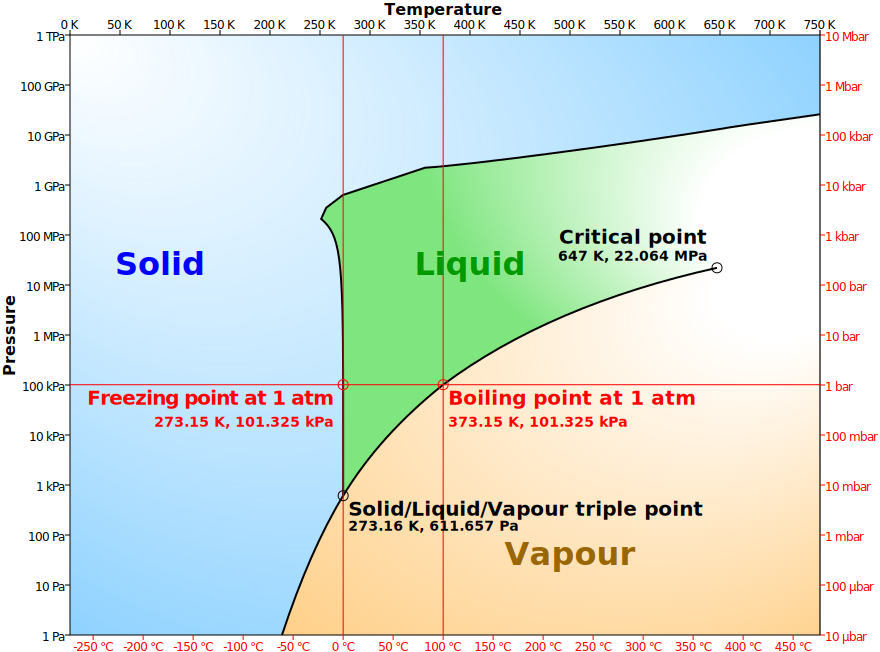
\includegraphics[width=0.7\linewidth]{bilder/Phase_diagram_of_water_simplified.pdf}
		\caption{Phasendiagramm von Wasser, Quelle: Cmglee nach LSBU}
	\end{figure}

	\note{
		\begin{itemize}
			\item[] Wasser kann in drei Phasen/Aggregatszuständen vorliegen: Gasförmig (Dampf), flüssig und fest (Eis)
			\item[] Besonderheit: Kommen alle drei in nennenswerter Menge in unserer Umwelt vor
			\item[] Phase hängt von Temperatur und Druck ab $\rightarrow$ Achsen des Phasendiagramms (Druck als log-Skala)
			\item[] Übergang von einer Pahsen zur anderen abrubt
			\item[] Punkte von besonderer Bedeutung:
			\begin{itemize}
				\item[] Schmelz- und Siedepunkt bei 1\, atm (Normaldruck) definierendie Celsius Temperaturskala
				\item[] Trippelpunkt: Punkt an dem Wasser in allen drei Phasen vorliegen kann (im thermodynamischen Gleichgewicht)
				\item[] Kritischer Punkt: Ab diesem Punkt gehen gasförmige und flüssige Phase in einander über
			\end{itemize}
		\item[] Dichteanomalie Besonderheit von Wasser
		\item[$\rightarrow$] Bei konstanter Temperatur kann die Phase von flüssig zu fest und wieder zu flüssig wechseln
		\item[$\rightarrow$] Wasser hat bei $\approx\SI{4}{\degreeCelsius}$ größe Dichte, darüber und darunter sinkt sie. Bei vielen anderen Stoffe steigt Dichte mit sinkender Temperatur
		\end{itemize}
	}
\end{frame}

\begin{frame}
	\frametitle{Interaktion Kryosphäre und Lithosphäre}

	\begin{figure}
		\centering
		\includegraphics[trim={1cm 0cm 0cm 3cm}, clip, width=0.55\linewidth]{%
				bilder/climate_components/global_climate_components_interaction_kryo_litho.pdf}
		\caption{Interaktion zwischen Kryosphäre und Lithosphäre}
	\end{figure}

	\note{
	\begin{itemize}
		\item[] An der Unterseite des Eisschildes, am Kontakt zwischen Fels und Eis, gibt es einen geothermischen Wärmeeintrag
		\item[$\rightarrow$] Temperatur entlang der Eissäule nimmt mit der Tiefe zu.
		\item[$\rightarrow$] Druckschmelzpunkt kann erreicht werden, sodass flüssiges Wasser an der Grenzschicht vorliegt.
		\item[$\rightarrow$] Schmierfilm, für den Eisschild, der zur schnellen Destabilisierung des westantarktischen Eisschildes führen kann.
		\item[] Weiterhin: Absenkung des Fels durch Gewicht des Eises um etwa \SI{30}{\percent} der Eisdicke
		\item[$\rightarrow$] Nordamerika und Skandinavien heben sich immer noch infolge der Entlastung der eiszeitlichen Eisschilde
	\end{itemize}
	}
\end{frame}

\begin{frame}
	\frametitle{Eis-Albedo-Rückkopplung}%Rahmstorf, Schellnhuber - Der Klimawandel S. 14
  \begin{center}
	 Reflexion der ankommenden Sonneneinstrahlung durch Eismassen\\[3em]
 \end{center}

	 \begin{columns}[T] % align columns
	 	\begin{column}{.48\textwidth}
	 		\centering
	 		\textbf{Abkühlung}\\
	 		\color{blue}\rule{\linewidth}{4pt}
	 		\color{black}
	 		\color<2->{gray}
	 		je mehr Eismassen\\
	 		$\downarrow$\\
	 		desto mehr wird reflektiert/\\
	 		desto weniger wird absorbiert\\
	 		$\downarrow$\\
	 		desto kälter wird es auf dem Planeten\\
	 		$\downarrow$\\
	 		desto weniger Wasserdampf kann die Atmosphäre aufnehmen\\
	 		$\downarrow$\\
	 		desto geringer wird der Treibhauseffekt
	 	\end{column}%
	 	\hfill%
	 	\begin{column}{.48\textwidth}<2->
	 		\centering
	 		\textbf{Aufwärmung}\\
	 		\color{red}\rule{\linewidth}{4pt}
	 		\color{black}
	 		je weniger Eismassen\\
	 		$\downarrow$\\
	 		desto weniger wird reflektiert/\\
	 		desto mehr wird absorbiert\\
	 		$\downarrow$\\
	 		desto wärmer wird es auf dem Planeten\\
	 		$\downarrow$\\
	 		desto mehr Wasserdampf kann die Atmosphäre aufnehmen\\
	 		$\downarrow$\\
	 		desto stärker wird der Treibhauseffekt
	 	\end{column}%
	 \end{columns}
\note{
\begin{itemize}
	\item[] Wechselwirkung unterschiedlicher Faktoren am Beispiel der Eis-Albedo Rückkoppelung
	\item[] Albedo ist im wesentlichen das Reflexionsvermögen eines Körpers auf einer Skala von 0 bis 1, eine hohe Albedo bedeutet viel Reflexion (Eis), eine niedrige Albedo bedeutet wenig Reflexion (Ozean)
	\item[] I.a. gibt es viele ähnliche Rückkoppelungen im Klimasystem, z.B. auch bei Landnutzung/Grünflächen und kann im Prinzip sowohl positiv wie negativ sein
	\item[] Negative Rückkoplung führt zu einem stabilen Verhalten, positive Rückkopplung zu schwer kontrolierbarem Anwachsen.
  \end{itemize}
  }

\end{frame}

% "Runterscrollen" / "Zoom" in einer Abbildung von den Atmosphärischen Schichten auf die Erde

\begin{frame}
	\frametitle{Interaktion Hydrosphäre, Kryosphäre und Atmosphäre}
	\begin{columns}
		\column{.6\linewidth}
		\begin{figure}
			\centering
			\includegraphics[trim={1cm 0cm 0cm 3cm}, clip, width=0.7\linewidth]{%
	        bilder/climate_components/global_climate_components_interaction_atmo_hydro_kryo.pdf}
			\caption{Interaktion Hydrosphäre, Kryosphäre und Atmosphäre}
		\end{figure}
		\column{.4\linewidth}
		\begin{itemize}
			\item Verringerter Albedo-Effekt
			\item Abgeschwächte Konvektion
			\item Abgeschwächte Ozeanströmung und Winde
			\item Anstieg des Meeresspiegels
			\item Massive Freisetzung von Treibhausgasen aus den Senken Ozean und Permafrost
			\item Trägheit führt zu verzögertem Eintreten der Änderungen
		\end{itemize}
	\end{columns}
	\begin{block}{}
			$\rightarrow$ Insgesamt: Eine Verstärkung des Treibhauseffekt mit weiteren noch unabsehbaren Folgen
	\end{block}

	\note{
		\begin{itemize}
			\item[] Verringerter Albedo-Effekt führt zu weniger Eis
			\item[] Wassermassen werden weniger stark abgekühlt, dadurch abgeschwächte Konvektion
			\item[] Ozeanströmungen und Winde werden ausgebremst
			\item[] Weniger Eis führt zu einem Anstieg des Meeresspiegels
			\item[] Massive Freisetzung von Treibhausgasen aus den Senken Ozean und Permafrost
			\item[] Trägheit führt zu verzögertem Eintreten der Änderungen
			\item[] Das Schmelzen der Polkappen und Auftauen des Permafrostes ist ein deutliches Signal
			\item[] Ein einmal in Gang gesetztes Abtauen kann schwer aufzuhalten sein
			\item[] Die Effekte können deutlich später auftreten (Trägheit der Klimakomponenten)
		\end{itemize}
	}
\end{frame}

\begin{frame}
	\frametitle{Interaktion Vegetation und Atmosphäre}

  \begin{figure}
    \centering
    \includegraphics[width=.55\linewidth]{bilder/Wind_Vegetation.jpg}
    \caption{Wechselwirkung zwischen Atmosphäre und Biosphäre, Quelle: Stadt Kriens}
  \end{figure}
		\begin{itemize}
			\item Bodenbedeckung wirkt auf Wind, Wasseraustausch und Strahlungshaushalt
			\item [$\rightarrow$] Wälder bremsen Winde, speichern Wasser, beeinflussen Wolkenbildung und bilden Schatten und großen Lebensraum
			\item [$\rightarrow$] in Wüsten und Steppen versickert Wasser schneller und es gibt kaum Schatten, dafür existiert schwacher Albedo-Effekt
			\item Existenz und Wachstum von Vegetation bindet u.a. CO$_2$ und absorbiert Strahlung
			\item Absterben von Vegetation führt zu Freisetzung von CO$_2$ und anderen Stoffen in die Luft und Böden % Nitrat, Phosphat, Stickstoff etc.
		\end{itemize}

	\note{
		\begin{itemize}
			\item[] Photosynthese: Aufnahme von CO$_2$ und abgabe von O$_2$, Nutzung des Kohlenstoff für das Wachstum
			\item[] Lösung organischer Kohlenstoff-Verbindungen durch baterielle Zersetzung $\rightarrow$ Freisetzung von CO$_2$
			\item[] Änderungen an der Landoberfläche durch z.B: Änderung der Landnutzung - Waldrodung, Landwirtschaft ändern auch die Vegetation und die Ökosysteme
		\end{itemize}
		Fragen? Sonst $\rightarrow$ Klimamodelle
	}
\end{frame}

%\begin{frame}
%	\frametitle{Interaktion Vegetation und Atmosphäre}
%
%		\begin{figure}
%		\centering
%		\includegraphics{bilder/WMO_Cycles_factors_landAndGround.png}
%		\caption{Interaktion der Biosphäre und Atmosphäre}
%	\end{figure}
%
%	\note{
%		\begin{itemize}
%			\item[] diesmal sind rechts die Wechselwirkungen der Vegetation und %Biosphäre zu sehen
%			\item[] links sind nochmal die zentralen Elemente der Komponente %Vegetation aufgelistet
%		\end{itemize}
%	}
%\end{frame}



\end{document}
